

  The following is an equilateral triangle of perimeter 12 inscribed inside a circle: \begin{center}
  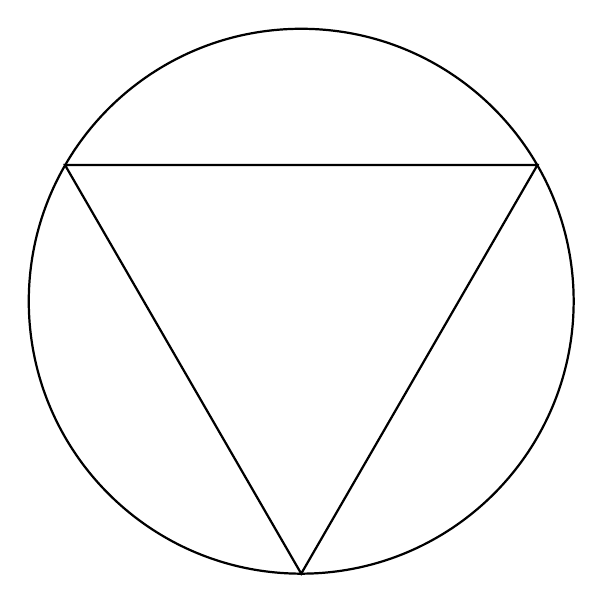
\begin{tikzpicture}[thick]



\draw[thick] (3,0)--(0,-3*1.73)--(-3,0)--cycle;

    \draw[thick] (0,-3*1.73/3) circle (3.46); 
                




  \end{tikzpicture}
\end{center}
How many equilateral triangles of perimeter 12 can you inscribe within this circle?


\ifsat
	\begin{enumerate}[label=\Alph*)]
		\item    2
		\item  3
		\item 4
		\item More than 4 %
	\end{enumerate}
\else
\fi

\ifacteven
	\begin{enumerate}[label=\textbf{\Alph*.},itemsep=\fill,align=left]
		\setcounter{enumii}{5}
		\item    2
		\item  3
		\item 4
		\addtocounter{enumii}{1}
		\item 8
		\item More than 4 %
	\end{enumerate}
\else
\fi

\ifactodd
	\begin{enumerate}[label=\textbf{\Alph*.},itemsep=\fill,align=left]
		\item    2
		\item  3
		\item 4
		\item 8
		\item More than 4 %
	\end{enumerate}
\else
\fi

\ifgridin
 More than 4 %

\else
\fi

